\header{
    \section{Le grenadier de Flandres} \label{le-grenadier-de-flandre}
    %
    
    \insertComment{Chanson traditionelle française antérieure au 18ème siècle.}{}
}

\enluminure{4}{\href{https://www.youtube.com/watch?v=l_gYdyrkwp4}{C}} \\
$\left.\begin{tabular}{l}
\hspace{-0.4cm}
\textsc{'était} un grenadier,
\\
\hspace{-0.4cm}
Qui revenait de Flandres,
\end{tabular}\right\rbrace$ bis
\\Qu'était si mal vêtu,
\\Qu'on y voyait son membre.
\\\\\textbf{Refrain :}
\\Le tambour bat,
\\La générale.
\bisdoublespace{La générale bat.}
{Le régiment s'en va.}
\\\bisdouble{Qu'était si mal vêtu,}
{Qu'on y voyait son membre.}
\\Un' dam' de charité
\\L'fit monter dans sa chambre
\\\bisdouble{Un' dam' de charité }
{L'fit monter dans sa chambre. }
\\Allum' cinq, six fagots
\\Pour réchauffer le membre.
\\\bisdouble{Allum' cinq, six fagots }
{Pour réchauffer le membre. ~~}
\\Quand le membre fut chaud,
\\Il se mit à s'étendre.
\\\bisdouble{Quand le membre fut chaud, }
{Il se mit à s'étendre.}
\\Aussi long que le bras,
\\Aussi gros que la jambe.
\\\bisdouble{Aussi long que le bras, }
{Aussi gros que la jambe. ~~}
\\"Dis-moi, beau grenadier,
\\A quoi te sert ce membre ?"
\breakpage
\\\bisdouble{"Dis-moi, beau grenadier,}
{A quoi te sert ce membre ?"}
\\"Il me sert à pisser,
\\Quand l'envie m'en vient prendre",
\\\bisdouble{"Il me sert à pisser, }
{Quand l'envie m'en vient prendre",}
\\"Et aussi à baiser,
\\Quand l'occasion s'présente."
\\\bisdouble{"Et aussi à baiser,}
{Quand l'occasion s'présente."}
\\"Eh bien, beau grenadier,
\\Fous le moi donc dans l'ventre".
\\\bisdouble{"Eh bien, beau grenadier,}
{Fous le moi donc dans l'ventre".}
\\"Ah! non, non, non, madame,
\\J'aurais peur de vous fendre".
\\\bisdouble{"Ah! non, non, non, madame,}
{J'aurais peur de vous fendre".}
\\"Fendue ou non fendue,
\\Il faut que tout y entre".
\\\bisdouble{"Fendue ou non fendue,}
{Il faut que tout y entre".}
\\La pine avec les couilles,
\\Il faut que tout y entre.
\\\bisdouble{La pine avec les couilles,}
{Il faut que tout y entre. ~~}
\\S'il en reste un p'tit bout,
\\Ce s'ra pour la servante.
\\\bisdouble{S'il en reste un p'tit bout,}
{Ce s'ra pour la servante.}
\\S'il n'en reste pas du tout,
\\Ell' se bross'ra le ventre.
\breakpage
\\\bisdouble{S'il n'en reste pas du tout,}
{Ell' se bross'ra le ventre.}
\\Elle ira dire partout :
\\"Madame est une gourmande".
\\\bisdouble{Elle ira dire partout :}
{"Madame est une gourmande".~~~~}
\\"Quand y-a d'la viande chez nous,
\\Ell' se fout tout dans l'ventre".
\\
\bigskip
\begin{center}
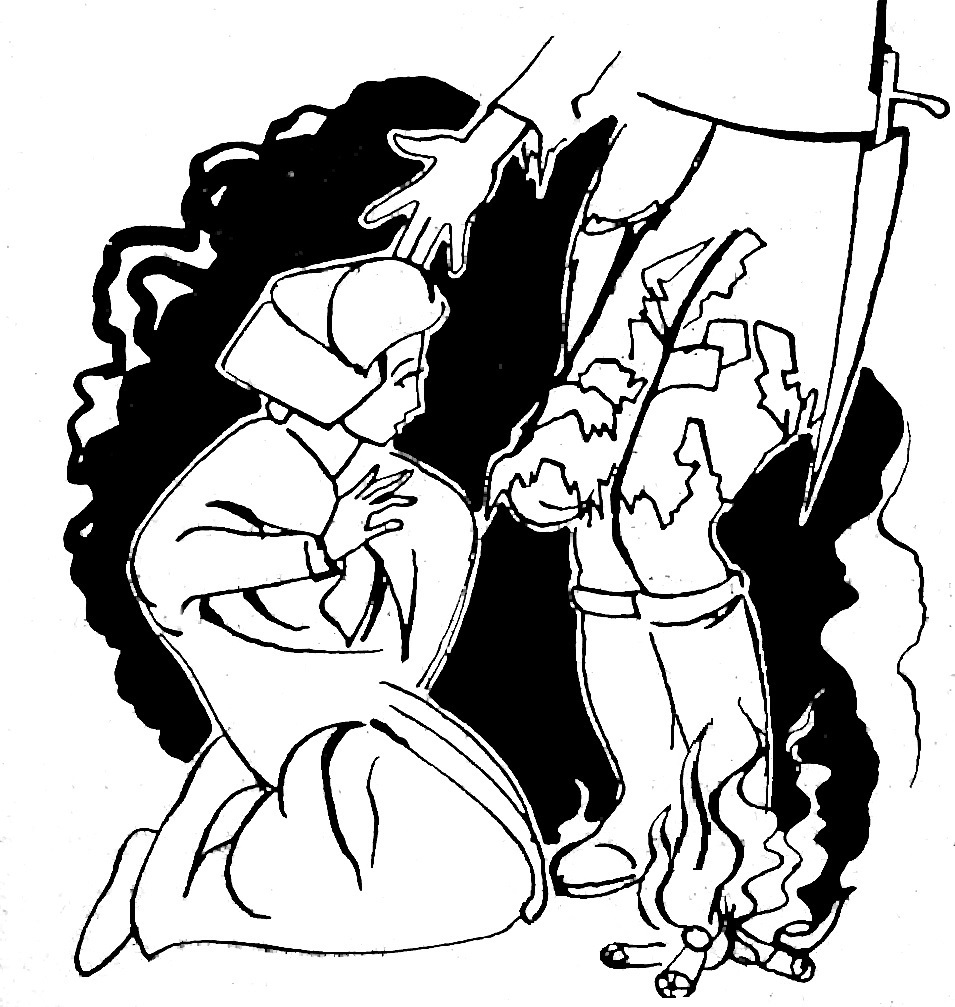
\includegraphics[width=1\textwidth]{images/grenadier.jpg}
\end{center}

\breakpage